\documentclass[11pt,dvipsnames]{article}

\usepackage{geometry}
\geometry{total={170mm,240mm}, left=20mm, top=20mm}

\usepackage[utf8]{inputenc}

\usepackage{physics} 
\usepackage{siunitx} 
\usepackage{enumerate} 
\usepackage{pgfplots}
\usepackage{graphicx}
\usepackage{pgfplotstable}
\usepackage{tikz,pgfplots}
\usepackage{amsmath} 
\usepackage{xcolor}
\usepackage{float}
\usepackage{amsfonts}
\usepackage{bbold}

\usepackage[]{lineno}  \linenumbers
\setlength\linenumbersep{3pt}
	

\usepackage{fancybox}
\usepackage{colortbl}
\usepackage{amsbsy}
\usepackage[draft,inline,nomargin]{fixme} \fxsetup{theme=color}
\FXRegisterAuthor{cp}{acp}{\color{blue}CP}
\FXRegisterAuthor{ja}{aja}{\color{RedViolet}JA}

\begin{document}

\title{Projective maps on a system of $n$ qubits} 
%Title should be concise and to the point  
\author{J. A. de León\\
				\small{supervised by C. Pineda}}


\date{\today}  

\maketitle


According to \cite{bengtsson_zyczkowski_2017}, an arbitrary density matrix on $n$  
qubits can be expanded as
\begin{align}
%	\rho = \frac{1}{2^n}\sum _{\vec{v}} \Tr 
%                  \qty( \sigma _{v_1} \otimes \sigma_{v_2} \otimes 
%               \cdots \otimes \sigma_{v_n} \rho) \sigma _{v_1} \otimes 
%             \sigma_{v_2} \otimes \ldots \otimes \sigma_{v_n},
  \rho = \frac{1}{2^n}\mathbb{1} + \sum _{i=1}^{2^{2n}-1}\tau _i\sigma _i,
	\label{rho}
\end{align}
where we'll identify $\sigma _i$ as the tensor products of Pauli 
matrices, which are a basis of the space of traceless density matrices, and 
$\tau_i$ the projections of $\rho$ onto each element of this particular
basis.

%where the sum is over vectors $\vec{v}=\qty(v_1,\cdots, v_n)$ with entries
%$v_i$ chosen from the set $\{0,1,2,3\}$. We label the coefficients $\Tr \qty(
%\sigma _{v_1} \otimes \sigma_{v_2} \otimes \cdots \otimes \sigma_{v_n}
%\rho )$ as $r_{v_1, v_2,\ldots, v_n}$ to shorten the notation. 
In this work, we are interested in studying the set of maps that erase
arbitrary components $\tau_i$ in $\rho$ and characterize the subset of maps
that are quantum channels. We'll refer to the coefficients in both terms of 
\eqref{rho} as the components in $\rho$.
%The kind of maps that act on density matrices of the form \eqref{rho} that
%we're interested in are those which leave invariant or erase  
%components
%in $\rho$ (i.e. $r'_{v_1, v_2,\ldots, v_n}=r_{v_1, v_2,\ldots, v_n}$ or
%$r'_{v_1, v_2,\ldots, v_n}=0$, where the primed $r$'s refer to the 
%components in the transformed density matrix $\rho '$). 

So far, with a numerical method we've characterized all 1 and 2 qubit maps, 
whereas for 3 qubits system we have numerically analized only maps that leave 
invariant 1, 2, 3, 4, and 64 components in $\rho$. Nonetheless, we have strong
indications that point that only the maps that leave invariant 8 components are 
needed to analyze in order to find the complete set of 3-qubit quantum 
channels.
\newline

\section*{Results}
In Figure \ref{fig:pictorial-rep-rho} we introduce a pictorial representation 
of an arbitrary density matrix for 1 and 2 qubits.
\begin{figure}[H]
	\centering
	\hfill \hfill
	
\includegraphics[height=2.5cm]
	{/home/deleonja/documents/docs_practicas/img-congreso/tablero-1q}
	\hfill
	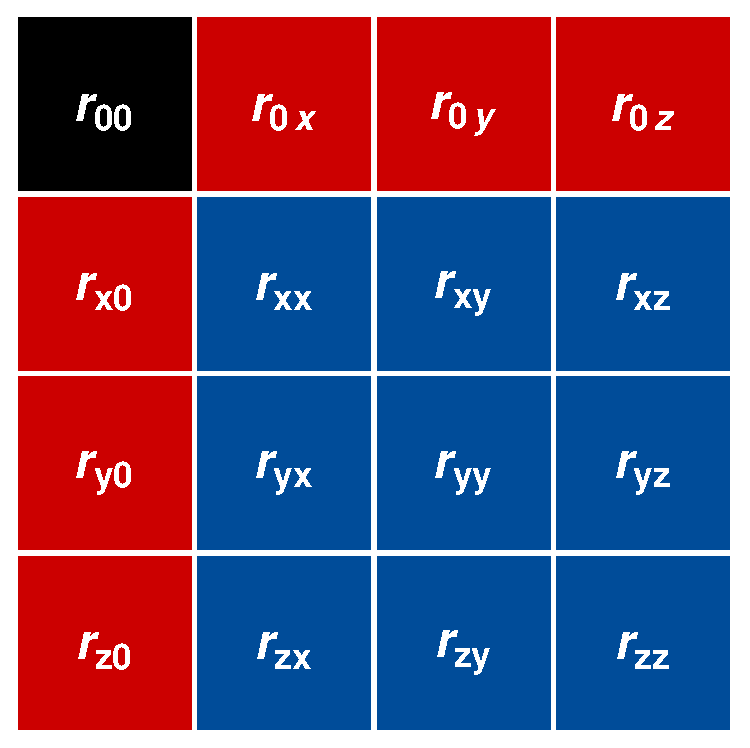
\includegraphics[width=2.5cm]
	{/home/deleonja/documents/docs_practicas/img-congreso/rho2q(2)}
	\hfill \hfill
	\caption{From left to right a pictorial representation for an arbitrary
	density matrix for 1 and 2 qubits, respectively. Red squares refer to local
	Bloch vectors and blue squared to the correlation matrix.}
	\label{fig:pictorial-rep-rho}
\end{figure}
In the following subsections we show the density matrices that result from
applying a quantum channel to an arbitrary density matrix in the representation
of Figure \ref{fig:CCs-by-components}.

\subsection*{1 qubit}
\begin{figure}[H]
	\centering
	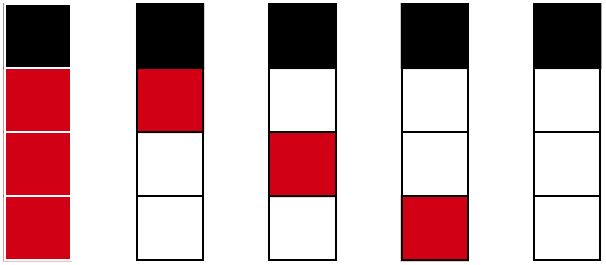
\includegraphics[width=5cm]
	{/home/deleonja/documents/docs_practicas/img-congreso/1q-CCs.png}
	\caption{1-qubit density matrices resulting from applying quantum channels
	to an arbitrary density matrix.}
\end{figure}

\subsection*{2 qubits}
\begin{figure}[H]
	\centering
  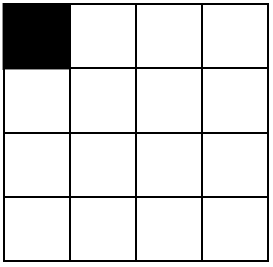
\includegraphics[height=1.2cm]
	{/home/deleonja/documents/docs_practicas/img-congreso/C16.png}
	\caption{C${}^{1}$}
\end{figure}

\begin{figure}[H]
	\begin{minipage}[c]{0.5\textwidth}
		\centering
	  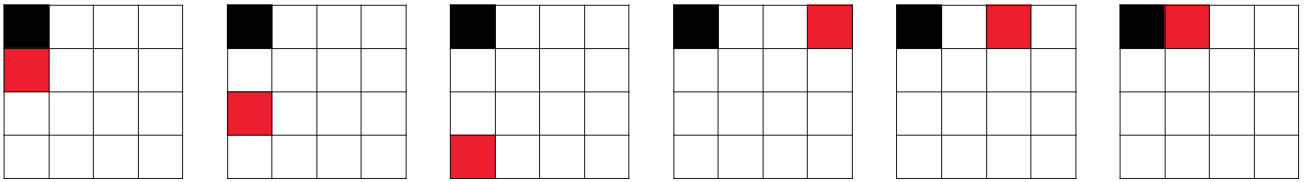
\includegraphics[width=.9\textwidth]
		{/home/deleonja/documents/docs_practicas/img-congreso/C12.png}
		\vspace{1.2cm}
		\caption{C${}_1^2$}
	\end{minipage}\hfill
	\begin{minipage}[c]{0.5\textwidth}
		\centering
	  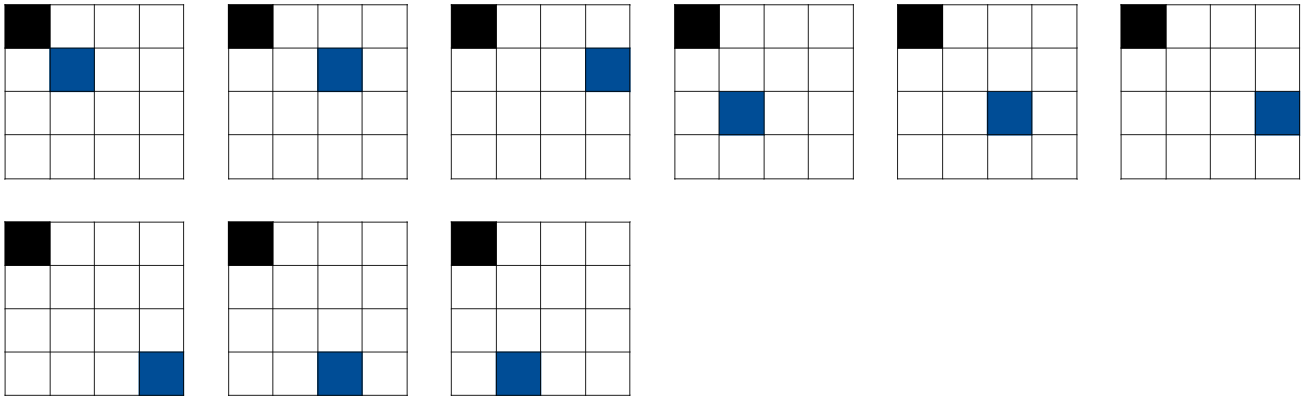
\includegraphics[width=.9\textwidth]
		{/home/deleonja/documents/docs_practicas/img-congreso/C22.png}
		\caption{C${}_2^2$}
	\end{minipage}
\end{figure}

\begin{figure}[H]
	\begin{minipage}[c]{0.5\textwidth}
		\centering
	  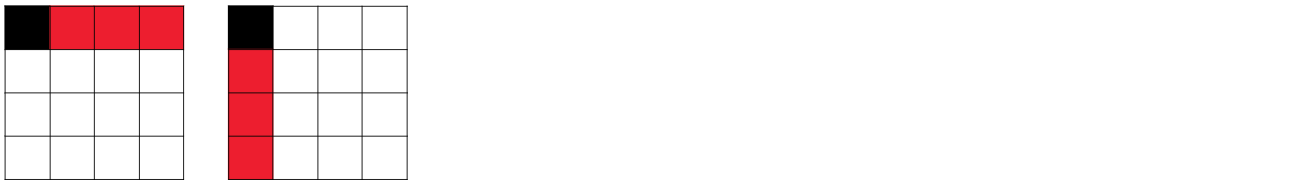
\includegraphics[width=.9\textwidth]
		{/home/deleonja/documents/docs_practicas/img-congreso/C14.png}
		\vspace{1.2cm}
		\caption{C${}_1^4$}
	\end{minipage}\hfill
	\begin{minipage}[c]{0.5\textwidth}
		\centering
	  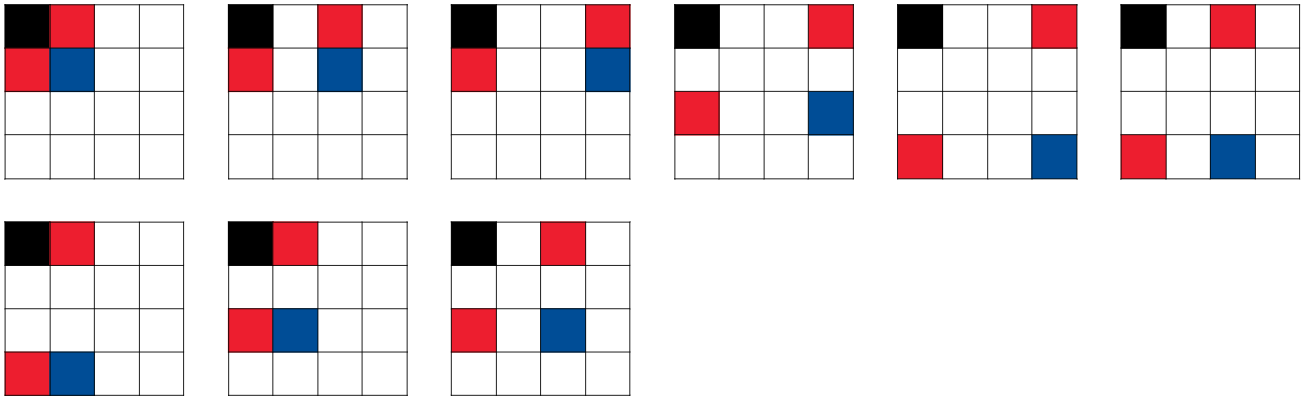
\includegraphics[width=.9\textwidth]
		{/home/deleonja/documents/docs_practicas/img-congreso/C24.png}
		\caption{C${}_2^4$}
	\end{minipage}\vfill
\begin{minipage}[c]{0.5\textwidth}
		\centering
	  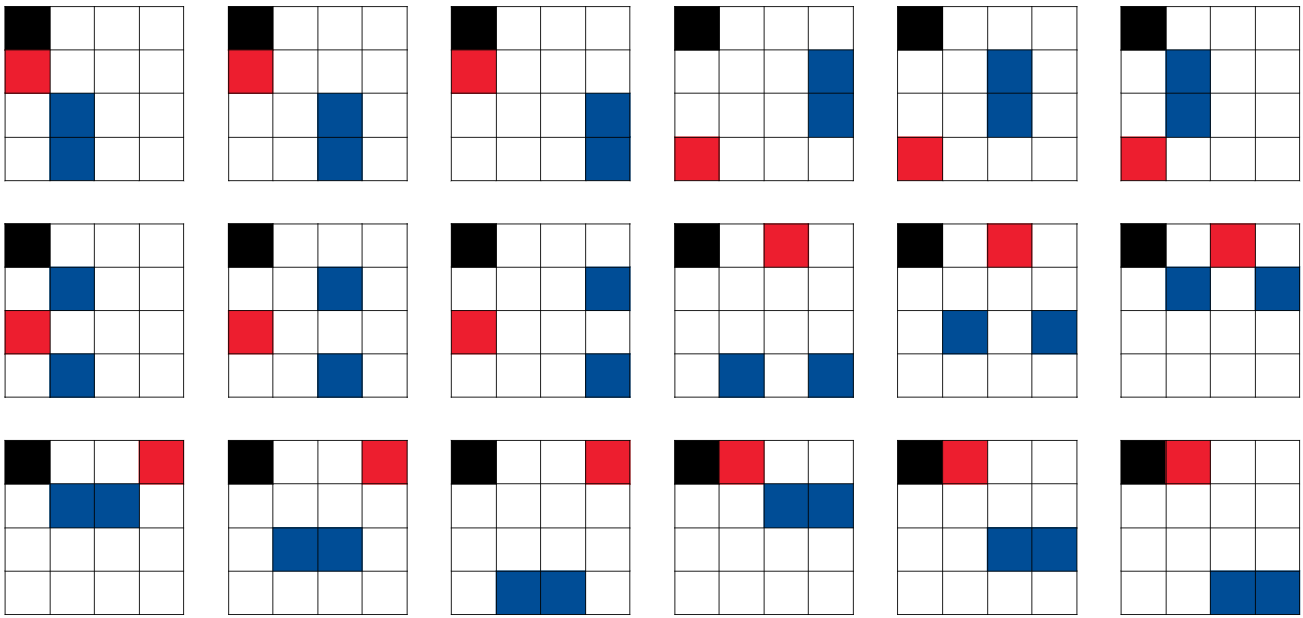
\includegraphics[width=.9\textwidth]
		{/home/deleonja/documents/docs_practicas/img-congreso/C34.png}
		\caption{C${}_3^4$}
	\end{minipage}\hfill
	\begin{minipage}[c]{0.5\textwidth}
		\centering
	  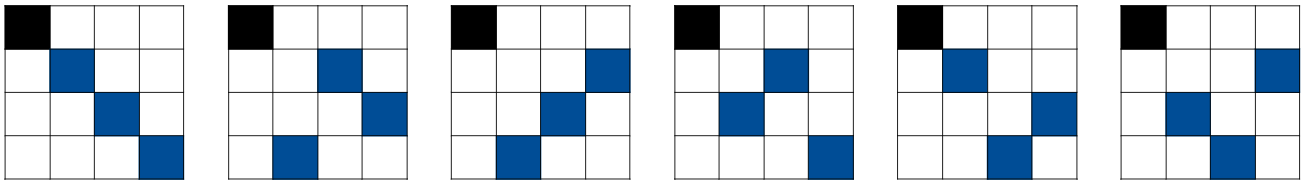
\includegraphics[width=.9\textwidth]
		{/home/deleonja/documents/docs_practicas/img-congreso/C44.png}
		\vspace{2.5cm}
		\caption{C${}_4^4$}
	\end{minipage}
\end{figure}

\begin{figure}[H]
	\begin{minipage}[c]{0.5\textwidth}
		\centering
	  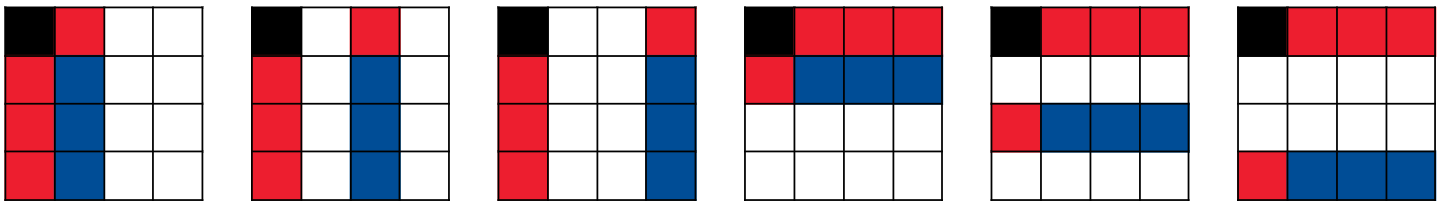
\includegraphics[width=.9\textwidth]
		{/home/deleonja/documents/docs_practicas/img-congreso/C18.png}
		\vspace{1.2cm}
		\caption{C${}_1^8$}
	\end{minipage}\hfill
	\begin{minipage}[c]{0.5\textwidth}
		\centering
	  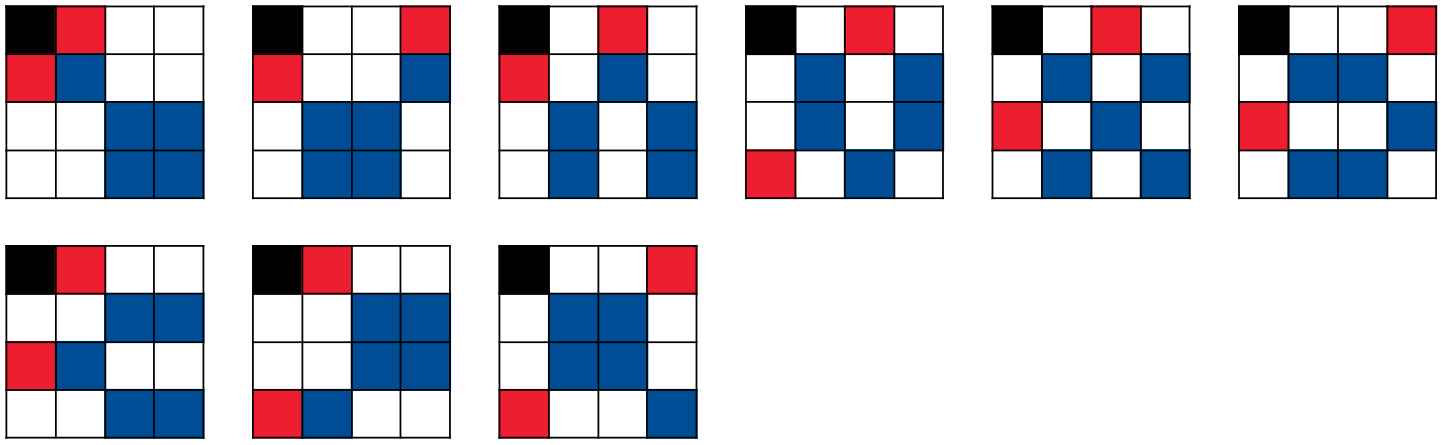
\includegraphics[width=.9\textwidth]
		{/home/deleonja/documents/docs_practicas/img-congreso/C28.png}
		\caption{C${}_2^8$}
	\end{minipage}
\end{figure}

\begin{figure}[H]
	\centering
  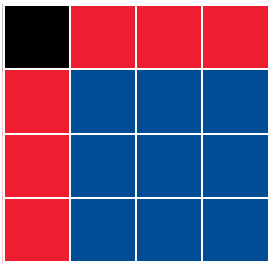
\includegraphics[height=1.2cm]
	{/home/deleonja/documents/docs_practicas/img-congreso/C0.png}
	\caption{C${}^{16}$}
\end{figure}

2-qubit results have been classified in equivalence classes (as shown) such
that elemtens in a class are conected by
\begin{enumerate}
	\item Transpotiions (particle swaps)
	\item Permutations of rows or columns 1-3 (permutation of individual 
	components)
\end{enumerate}

In general, our results exhibit the following features:
\begin{itemize}
\item Only a power-of-2 number of components may be left invariant by 
			quantum channels. However,
			not only the number of 
			coefficients to leave invariant is taken into account but actually
			which coefficientes are left invariant too.

\item 
The number of valid quantum channels according to the number of components
left invariant are shown in Figure \ref{fig:CCs-by-components}. Two numbers
of same color correspond to quantum channels that we suspect have a 1:1 
correspondence. In the next item we extend this discussion.

\begin{figure}[H]
	\centering
		\begin{tabular}{>{$n=}l<{$\hfill}*{12}{c}}
			1 &&&&&\colorbox{Apricot}{1}&3&\colorbox{Apricot}{1}&&&&&5\\
			2 &&&&\colorbox{CadetBlue}{1}&\colorbox{Cyan}{15}&35&\colorbox{Cyan}{15}&\colorbox{CadetBlue}{1}&&&&67\\
			3 &&&\colorbox{SpringGreen}{1}&\colorbox{RedOrange}{63}&\colorbox{Yellow}{561}&?&\colorbox{Yellow}{¿561?}&
				\colorbox{RedOrange}{¿63?}&\colorbox{SpringGreen}{1}&&&?
			\end{tabular}
			\caption{First column shows the number of qubits in the system. 
							In the second column each position correspond to the 
							number of components invariant ($2^0, 2^1, \ldots, 2^{2n}$) and
							the numbers shown are the number of quantum channels according to 
							the number of components invariant.
							Finally, third column specifies the total number of quantum 
							channels for a n-qubit system.}
			\label{fig:CCs-by-components}
\end{figure}

\item Empirical observations of 2-qubit results led us to some rules that 
			patterns in Figures obey:
			\begin{enumerate}
				\item If a component with indices $ij$ is left invariant, then two 
							options are allowed: \textit{a.} both components with indices $i0$ 
							and $0j$ are left invariant too, or \textit{b.} both
							components with indices $i0$ and $0j$ are erased.
				\item Focusing only on the correlation matrix (blue squares): if a 
							component	with indices $ij$ is left invariant and the previous 
							rule is obeyed, then the reamining components in the correlation 
							matrix on row $i$ and column $j$ must be erased.
			\end{enumerate}	Actuallly, this two simple rules allow us to connect
			two elements of classes C${}^2_k$ and C${}^8_k$.

%For 3 qubits the maps that leave invariant 16 components in $\rho$
%have not been numerically analized, but we pressume there's a 
%1-on-1 correspondence for the number of valid channels between those that leave
%invariant 2 and 32 components, and similarly between those that leave 4 and 16
%componentes invariant. This observation follows 
%from the correspondence in the results for 1 and 2 qubits 
%between quantum channels that leave invariant $2^k$ and $2^{2n-k}$, for 
%$k=1, 2, \ldots, n$.
		
% \item The results are recursive by increasing the number of qubits in the
% system, i.e. the valid quantum channels for 2 qubits have to obey the valid
% quantum channels for 1 qubit. In more detail, 
%\item Valid maps for $n$ qubits must be valid for subsets of qubits. For example,
%the 2-qubits quantum-channels
%that leave invariant any of the coefficients of the form $r_{v_1,0}$ or
%$r_{0,v_2}$ have to obey the valid quantum channels found for 1 qubit. 
%This induces nice rules that are not accessible (we think) by considering 
%a single $2^n$-level quantum system. {\color{blue} [Nota]
%No entiendo la utilidad de este punto. Salvo la regla que nos permite ver si el canal es un producto tensorial de canales (o no), no se a que otras reglas se refieren. Claramente un producto tensorial de canales es tal que los 1s internos coinciden con los 1s en las orillas. Si se especificará mas este punto, propongo borrarlo, creo que mete ruido.}

%\janote{A mí no me convence la redacción del item anterior. A diferencia de 
%				David, a m\'i s\'i me parece una observaci\'on importante porque evidencia
%				que nuestros canales deben respetan las acciones v\'alidas sobre todos los 
%				subsistemas, as\'i el canal no sea factorizable.}
%
%	\item One can identify that $r_{v_1,v_2,\ldots,v_n}$ is composed from the 
%				individual Bloch vectors of each qubit and the correlation tensors of
%				every system's subset. Then, with the action of a quantum channel in 
%				terms	of $r'_{v_1,v_2,\ldots,v_n}$ in mind, quantum channels are found
%				for those whose action on an arbitrary $\rho$ reproduce valid 
%				results in every of the components of $r'_{v_1,v_2,\ldots,v_n}$.

	\item The action of a quantum channel on every subsystem must be another
				channel.

%	\item Separable quantum channels are those constructed from the tensor product
%				of valid quantum channels for subsets of qubits in the system that
%				that follow the 
%				power-of-2 rule for the components left invariant in $\rho$. For 2
%				qubits, 25 quantum channels are of this particular type (this is the
%				number of permutations with repetition of the five 
%				quantum channels of 1 qubit). Therefore, the remaining 42 channels
%				cannot be infered with the information provided by the 1-qubit
%				quantum channels, in principle.
\end{itemize}

We explored if the kind of quantum channels of our study are a subset 
of the Pauli diagonal channels constant on axes \cite{nathanson2007pauli}.
We were unable to demonstrate in a irrefutable manner that 
our quantum channels are not a particular case of channels constant on axes, 
but we strongly suspect that they're not. We briefly discuss this in the 
next parragraph. 

Let's consider any density matrix written as
\begin{align}
	\rho = \frac{1}{d}\qty[\mathbb{1} + \sum _{J=1}^{d+1} \sum _{j=1}^{d-1}
	v_{Jj}W_J^j],
	\label{eq:ruskai-rho}
\end{align}
where $d$ is the dimension of the Hilbert space of the system and $W_J^j$ 
are generators of a mutually unbiased bases (MUB) for $\mathbb{C}^{d}$. Then,
the action of a Pauli diagonal channel constant on axis on a $\rho$ of the form
\eqref{eq:ruskai-rho} is to take $v_{Jj}\mapsto (s+t_J)v_{Jj}$. Using a few
different sets of tensor product of Pauli matrices that generate MUB's for
$\mathbb{C}^4$, listed in section 12.4 of \cite{bengtsson_zyczkowski_2017}, 
we noted that a particular case of this maps, if it is to coincide with our subject of
study, must be such that it leaves invariant $1+3k$ components ($k$ an integer)
in $\rho$. Therefore, for a 2-qubit system quantum channels that leave 
invariant 2 and 8 components cannot be repdroduced by maps constant on axes. 

\section*{To-do}
In order to fully understand our results and generalize this kind of maps 
for $n$ qubits is the following:
\begin{enumerate}
	\item Investigate the Kraus operator representation of this quantum channels.
	\item Investigate the Schmidt spectrum of the Choi matrix.
	\item Investigate the Jamiolkowski isomorphism to find an equivalence
				between CP and the empirical rules listed previously.
	\item Use our current results to propose an efficient way to do numerical
				analysis to find 3-qubit quantum channels that leave 8 components 
				invariant.
\end{enumerate}

\bibliographystyle{unsrt}
\bibliography{references}
\vfill

\end{document}
